\documentclass[sigconf]{acmart}

% Author-review proof: eRights, author name, email and ORCID confirmed by author.
\settopmatter{printacmref=true,printccs=true,printfolios=true}
\usepackage{booktabs}
\usepackage{microtype}
\usepackage{balance}
\emergencystretch=1em

% Exact publication metadata supplied in the author's ACM eRights confirmation.
% The private form link is intentionally not stored in the manuscript source.
\copyrightyear{2026}
\acmYear{2026}
\setcopyright{cc}
\setcctype{by}
\acmConference[HAI '26]{Proceedings of the 14th International Conference on Human-Agent Interaction}{November 16--19, 2026}{Osaka, Japan}
\acmBooktitle{Proceedings of the 14th International Conference on Human-Agent Interaction (HAI '26), November 16--19, 2026, Osaka, Japan}
\acmDOI{10.1145/3841580.3845761}
\acmISBN{979-8-4007-2575-3/2026/11}


\title{From Shelf Order to Later Agent Choice: A Link-by-Link Audit of Recommendation Writeback}
\author{Kaiqi Feng}
\orcid{0009-0006-1970-9572}
\affiliation{%
  \department{College of Design and Innovation}
  \institution{Tongji University}
  \city{Shanghai}
  \country{China}}
\email{2354251@tongji.edu.cn}

\begin{CCSXML}
<ccs2012>
<concept><concept_id>10002951.10003260.10003277</concept_id><concept_desc>Information systems~Recommender systems</concept_desc><concept_significance>500</concept_significance></concept>
<concept><concept_id>10003120.10003121.10003129</concept_id><concept_desc>Human-centered computing~Interactive systems and tools</concept_desc><concept_significance>300</concept_significance></concept>
</ccs2012>
\end{CCSXML}
\ccsdesc[500]{Information systems~Recommender systems}
\ccsdesc[300]{Human-centered computing~Interactive systems and tools}
\keywords{human-agent interaction, delegated agents, recommender systems, recommendation order, writeback}

\begin{document}

\begin{abstract}
When an AI shopping agent selects a product, that choice may shape what the
platform recommends next. Yet the choice itself may already reflect how the
platform arranged the products. We ask whether this influence remains visible
after the selected item enters account history. In a research storefront with
460 constructed tasks, two sequential recommenders, and two LLM providers, we
trace this process one link at a time. Reordering identical candidate records
changed immediate choices. Writing those selections into history then produced
small, measurable differences in later shelves and later agent choices for
both providers. An extension using ordinary-language shopping tasks also found
order-sensitive choices. These findings motivate separating task-local
assistance from decisions about what enters account history. The study follows
one step of model--recommender feedback; whether it amplifies over repeated
interactions remains unresolved.
\end{abstract}

\maketitle

\section{Introduction}

A shopping agent sees an ordered shelf. Once stored in account history, its
choice may alter later shelves. LLM order effects and agentic commerce are
established \cite{bito2025position,allouah2025agentbuying,zhang2026ranked}.
ABxLab tests attribute and nudge effects in agent shopping
\cite{cherep2026abxlab}; recommender work traces position-biased feedback into
item popularity \cite{dzhoha2024position}. Agent4Rec, AFL, RecInter, and
RecLoop further model feedback between simulated agents and recommenders
\cite{zhang2024agent4rec,cai2025afl,jin2025recinter,yang2026recloop}. These
systems study interaction over time. We focus on a specific transition:
whether an order-only difference remains visible after the selected item is
written back and a learned recommender produces the next shelf.

Our experiment separates the initial order effect from its consequence for
later input. First, candidate identities and attributes stay fixed while order
changes. Next, the selected item enters history as a standardized event; the
recommender generates a later shelf for another categorical choice.
Selected-item identity can now differ between arms: this second contrast
follows a mediated path rather than another order-only intervention
(Figure~\ref{fig:chain}).

\begin{figure*}[t]
  \centering
  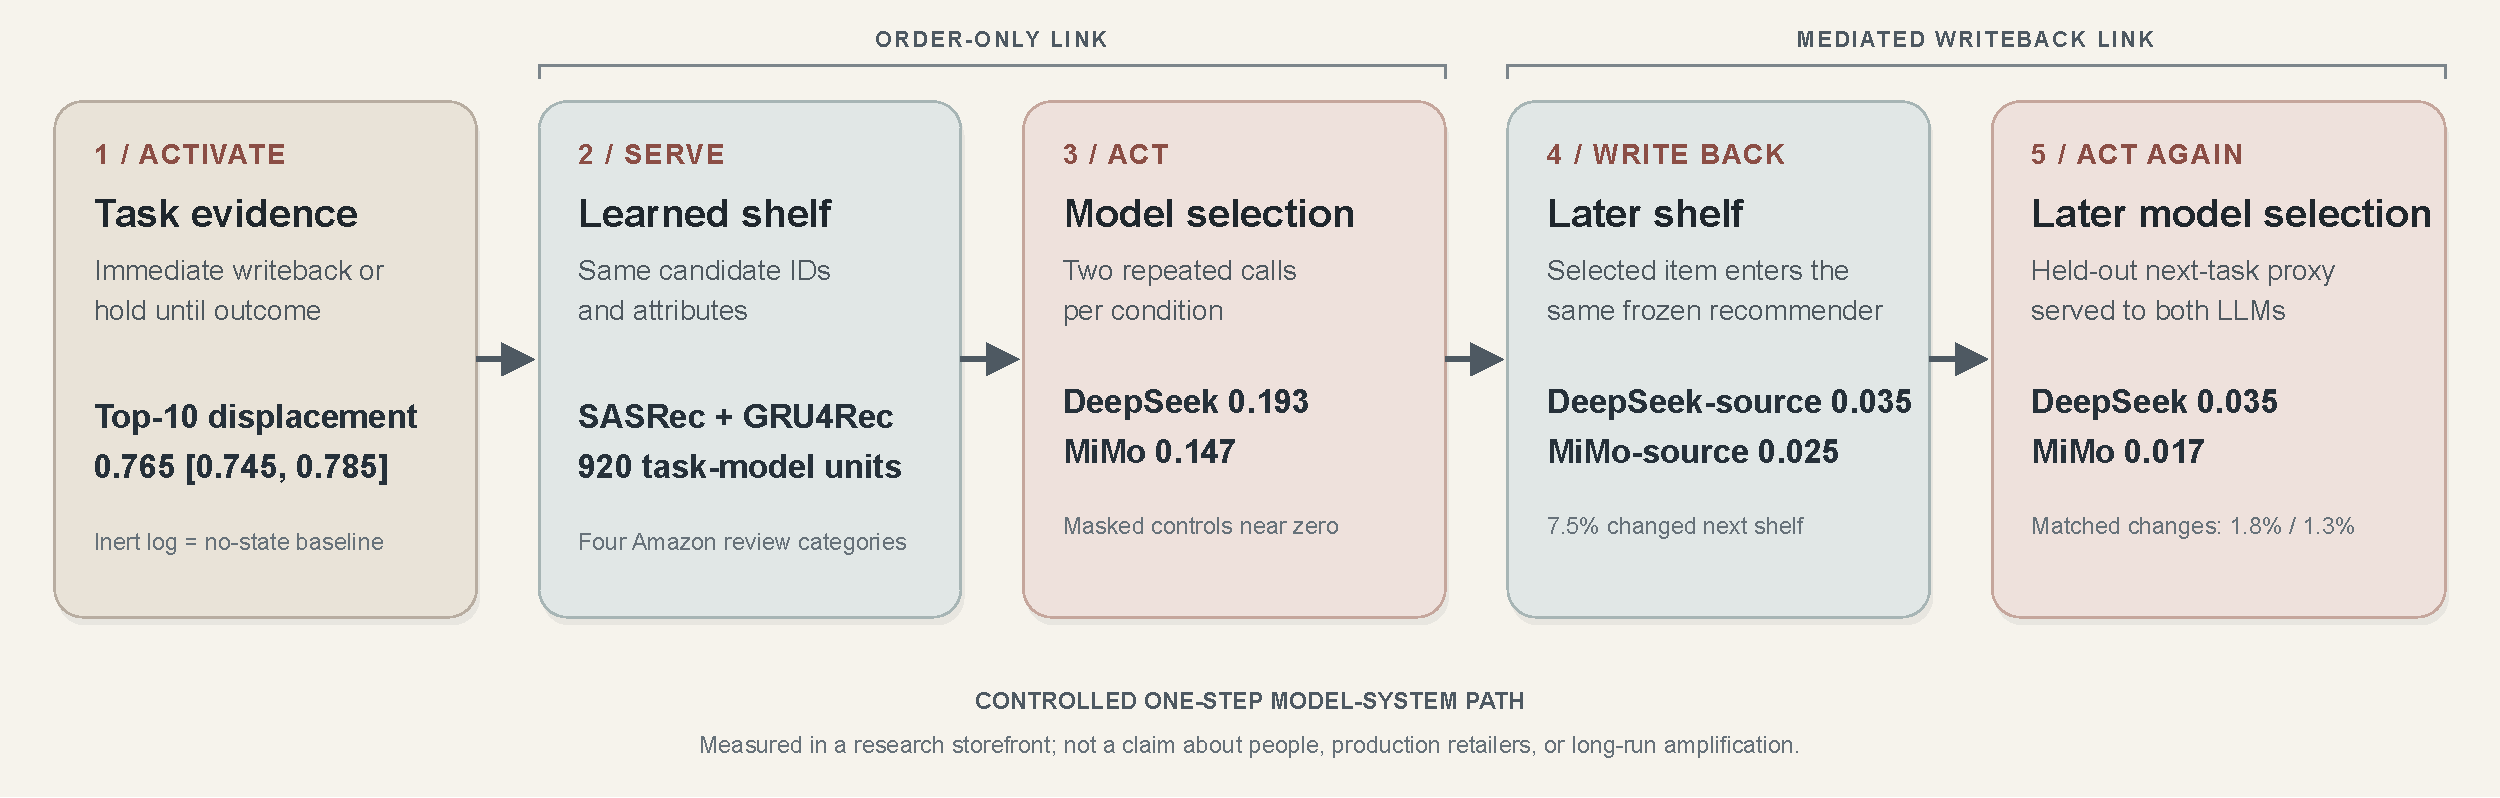
\includegraphics[width=\textwidth,height=143pt,keepaspectratio]{figures/feedback-chain-restored.pdf}
  \caption{Measured path from shelf order to later agent choice. The order-only
  link fixes candidate identity and attributes; the mediated writeback link
  follows the selected item through one later shelf and choice.}
  \Description{A five-stage horizontal chain on a cream background. Stage 1,
  Activate, contrasts immediate writeback with holding task evidence until the
  outcome and reports top-10 displacement of 0.765 with a 95 percent interval
  from 0.745 to 0.785. Stages 2 and 3 are grouped as the order-only link. Stage
  2 serves learned shelves from SASRec and GRU4Rec across 920 task-model units
  while preserving candidate identities and attributes. Stage 3 measures model
  selection, with adjusted choice distances of 0.193 for DeepSeek and 0.147 for
  MiMo; masked controls are near zero. Stages 4 and 5 are grouped as the
  mediated writeback link. Stage 4 writes the selected item into the same
  frozen recommender and reports later-shelf distances of 0.035 for
  DeepSeek-source choices and 0.025 for MiMo-source choices, with 7.5 percent of
  next shelves changed. Stage 5 serves a held-out next-task proxy and reports
  later-choice distances of 0.035 for DeepSeek and 0.017 for MiMo, with matched
  choice changes of 1.8 and 1.3 percent. The figure describes a controlled
  one-step model-system path, not people, production retailers, or long-run
  amplification.}
  \label{fig:chain}
\end{figure*}

\section{Research Storefront and Protocols}

We built 460 tasks, 115 per category, from four public Amazon Reviews 2018
sequences \cite{ni2019amazon}. Study 1 used frozen SASRec checkpoints
\cite{kang2018sasrec}. Studies 2 and 3 crossed every task with SASRec and
GRU4Rec \cite{hidasi2016gru4rec}, producing 920 task-model units. During model
calls, the LLMs received pseudonymous IDs and derived scalar features instead
of titles, histories, or review text. DeepSeek V4 Flash and MiMo V2.5 ran at
temperature zero in August 2026. The frozen protocol assigned DeepSeek the
primary contrast and MiMo a second-provider replication across available API systems.
Supplementary Material S1 includes complete cached prompt examples,
provider-specific wrappers, output constraints, and a paired-input audit;
the computational artifact retains protocols, code, and result primitives.

\textbf{Study 1: activation.} We replayed the same behavior and candidate masks
while changing whether temporary task events were logged or activated in the
learned recommender. This comparison isolates recommender activation from event
recording.

\textbf{Study 2: order to action.} For every unit and provider, we used four
input constructions: rank metadata only, inspection state only, a
byte-identical masked control, and served order. The served-order comparison
kept candidate IDs and attributes fixed and changed only their order. Within
each provider, system instructions, task text, serialization, output constraints,
and decoding settings stayed fixed across arms. Each arm
received two calls, yielding 29,440 valid responses. We used the categorical
energy construction \cite{szekely2013energy}: twice cross-arm disagreement
minus the two within-arm disagreements. Under stable, independent, exchangeable
calls, its mean task-conditional U-statistic estimates squared $L_2$ distance
between categorical output distributions. Two-call unit estimates are noisy
and may be negative. We formed intervals by resampling tasks within category
while retaining both recommender families and every mode. We froze these rules
and the controls before running the study.

\textbf{Study 3: writeback.} We appended each Study 2 selection to the same
frozen recommender history as a standardized positive event. We then added one
held-out next event and generated a new Top-10. The source provider received
this later shelf with a held-out next-task proxy. Each provider retained all
920 units. Within category, recommender, and mode strata,
a frozen four-row cyclic Latin square assigned the four semantic conditions to
call positions; counts differed by at most one. The same 226
protocol-hash-selected units received a byte-identical downstream control.

\textbf{Product-language extension.} In 64 tasks crossed with both recommenders
(128 units; 60 with a feasible offered item), both providers saw
ordinary-language requests and the same 12 cleaned title, brand, and price
records in arm-specific order. We scored task outcomes privately and continued
each trajectory for three fixed steps. The continuation compared selected
events with one deterministic random realization matched on write count and
whether paired writes were equal.

\section{Results}

Logging without activation did nothing. Immediate activation versus holding produced a mean
in-task Top-10 displacement of 0.765 [0.745, 0.785], while no-state and
inert-log shelves agreed. At resolution and the standardized next task, fixed
replay returned to zero displacement.

Order-only exposure changed categorical choices for both providers.
DeepSeek's distance was 0.193 [0.151, 0.239], compared with 0.004 [-0.003,
0.013] in the masked control. MiMo's distance was 0.147 [0.110, 0.187], versus
0.000 [-0.007, 0.008] in its control. All cross-arm changes were swaps between
selectable candidates, not select-to-abandon transitions.

The selected-item difference remained measurable after writeback.
DeepSeek-sourced selections produced later-shelf distance 0.035 [0.024,
0.047]; MiMo-sourced selections produced 0.025 [0.016, 0.035]. Estimates were
positive for SASRec (0.018 [0.010, 0.027]) and GRU4Rec (0.052 [0.034, 0.071]).
Serving later shelves back to their source provider produced distances
0.035 [0.017, 0.054] for DeepSeek and 0.017 [0.005, 0.032] for MiMo; both
226-unit byte-identical controls were zero. Matched repeat-pair change rates were 1.8\%
[1.0\%, 2.8\%] (34/1,840 comparisons; 18/920 units with any change) and 1.3\%
[0.7\%, 2.0\%] (24/1,840; 15/920 units). MiMo's SASRec-only
estimate was 0.007 [-0.004, 0.020], while GRU4Rec was 0.028 [0.009, 0.052].

Across the 128 product-language units, DeepSeek and MiMo order distances were
0.309 [0.180, 0.453] and 0.289 [0.180, 0.414]. Success differences (holding minus immediate)
were 0.031 [-0.008, 0.078] and 0.023 [-0.016, 0.066]; regret and failure also
included zero. At step three, the selected-versus-random difference was 0.007
[-0.023, 0.035] for DeepSeek. For MiMo it was -0.017 [-0.036, -0.001]. Point
estimates did not consistently favor selected writeback, but one random
realization cannot establish equivalence or absence of amplification.

\section{Implications and Limits}

The chain identifies two design decisions: how the platform presents candidates,
and when an agent's selection becomes account history. Prior systems separate intent-specific
profiles \cite{tsukuda2025intent}, recommendation memories
\cite{zhan2026calmrec}, memory admission \cite{xiong2026memory}, or agents from
platforms \cite{xu2025iagent}. Our study follows an order-induced choice through
one writeback cycle. This motivates an interface that separates task-local
assistance from admission to account history, with task outcome informing that
admission. Evaluating that design requires a direct policy comparison and
measures of the principal's goals.

The evidence concerns model--recommender behavior, with no human participants.
Tasks and next-task targets are constructed proxies; token-and-price success
is not human utility. Later pilot steps use a fixed policy rather than repeated
LLM calls. Two available providers are not representative of LLMs, and two
repeats per arm limit stationarity assessment. DeepSeek returned one provider
fingerprint; MiMo returned none. The one-step horizon and 1.3--1.8\% matched
endpoint rates establish neither human harm nor long-run amplification.

\paragraph{Generative AI disclosure.} Generative AI tools assisted with code
generation, experiment orchestration, and language editing. The author checked
the protocols, statistical decisions, sources, and reported results against the
frozen artifacts included with the submission.

\balance
\bibliographystyle{ACM-Reference-Format}
\bibliography{references}

\end{document}
